\documentclass{GSHS-chemexp}

\begin{document}
	
	\title{질량 측정과 액체 옮기기}	
	\date{2015. 03. 06 (금)}
	\coauthor{14020 김유빈, 14104 정재석}
	\author{14088 이주찬}
	\maketitle
	
	\section{실험 개요}
	
	\subsection{실험 목적}
	
	\begin{itemize}
		\item 화학 실험의 기본이 되는 저울 사용법과 액체를 옮기거나
		부피를 측정할 때 사용하는 기구의 조작법을 익힌다.
		\item 실험 데이터의 처리 및 불확정도 추정 방법을 이해한다.
	\end{itemize}
	
	\subsection{이론적 배경}
	
	\subsubsection{유리 기구의 눈금 읽는 방법}
	유리 기구의 눈금이 새겨진 부분이 수직이 되도록 세운 뒤
	눈금을 읽어야 하고, 액체를 넣은 뒤 \unit{1}{분} 이상 기다려서
	유리 벽에 묻은 액체가 모두 흘러내린 뒤 눈금을 읽어야 한다.
	눈금을 읽을 때는 눈높이를 액체의 메니스커스에 맞추고,
	메니스커스의 밑바닥 부분에 해당하는 위치를 읽는다.
	단, 유리 기구에 담긴 액체가 유리와 반발하는 경우(수은 등)는
	메니스커스의 윗부분을 읽는다.
	눈금은 가장 작은 눈금을 10 등분 하여 읽는다.
	즉, 최소 눈금 단위가 \SI{1}{\milli\litre}인 유리 기구의
	눈금을 읽을 때는 \SI{0.1}{\milli\litre}까지 읽어야 한다.
	\begin{figure}[H]
		\centering
		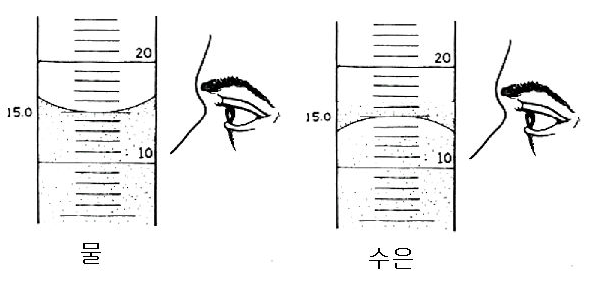
\includegraphics[width=0.7\textwidth]{Meniscus.png}
		\caption{물과 수은의 메니스커스 읽는 방법}
		\label{fig:meniscus}
	\end{figure}
	
	\subsubsection{측정의 불확실성}
	
	\paragraph{정밀도와 정확도}
	화학은 실험 과학이므로 모든 정량적 측정은
	어느 정도의 오차를 가진다.
	측정을 여러 번 반복하거나 실험 기구를 바꿈으로써
	오차를 줄일 수는 있지만, 완전히 오차를 제거할 수는 없다.
	그러므로 실험 측정값의 타당성 한계를 설정하기 위해서는
	실험 결과를 정량적으로 평가하는 것이 중요하다.
	오차는 두 가지 형태로 나타나며 이들은
	정밀도의 부족(우연 오차, random error)과
	정확도의 부족(계통 오차, systematic error)에 기인한다.
	\begin{figure}[H]
		\centering
		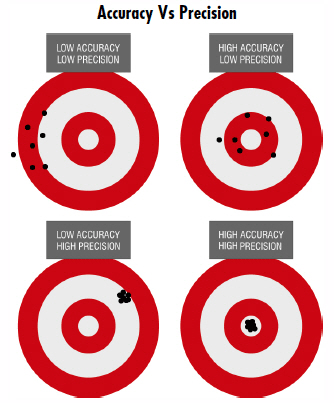
\includegraphics[width=0.5\textwidth]{Accuracy_Precision.jpg}
		\caption{정확도와 정밀도의 차이}
		\label{fig:acc_pre}
	\end{figure}
		
	\paragraph{정밀도와 우연 오차}
	정밀도란 측정한 실험 결과 간에 일치하는 정도를 나타내는 것으로
	가능한 한 같은 조건에서 측정을 반복하여 결정한다.
	만약 조건이 똑같다면 측정값 간의 차이는 우연 오차에 기인한다.
	실험으로 얻은 결과 중 가장 적합한 결과를 취하기 위해서는
	먼저 나머지 값들과 유난히 차이가 크게 나는 값을 제외한 다음
	(측정이나 기록의 실수일 수 있으므로)
	측정값의 평균을 대푯값으로 취한다.
	측정을 반복해서 할 수록 우연 오차에 의한 측정의 불확도는 줄어들게 된다.
		
	\paragraph{정확도와 계통 오차}
	계통 오차란 측정값이 참값으로부터 원천적으로 벗어나게 하여
	측정값의 정확도를 감소시킨다.
	우연 오차에 기인한 불확실성은 측정 횟수를 늘림으로써
	줄일 수 있고 결과의 정밀도를 향상시킬 수 있다.
	그러나 계통 오차가 있으면 평균값은 참값과
	계속 일치하지 않을 것이고 그러한 계통 오차는
	실험 기구의 잘못된 눈금, 또는 특성을 측정하려는 기술의
	근본적인 부적절함에 기인할 수 있다.
	그러므로 정확도의 부족은 정밀도의 부족보다 훨씬 해결하기 곤란하다.
	
	계통 오차가 있는 것으로 확인되면 측정값을 결정하기에 앞서
	계통 오차를 제거하여야 한다.
	(예를 들어, 실험 기구의 눈금이 정확하지 않으면
	다시 눈금을 만들어야 한다)
	문제는 알지 못하는 계통 오차가 있을 수도 있다는 것이며
	이러하다면 한 특정 부분의 장치에 기인한 계통 오차를
	제거하기 위해 다른 기구를 가지고 실험을 반복해야 한다.
	
	\subsubsection{측정의 불확실성과 유효숫자}
	어떠한 측정이건 간에 측정의 불확실성을 나타내는 것은 매우 중요하다.
	측정한 결과는 언제나 약간의 불확실성을 포함하고 있으며
	불확실성의 수치는 측정 장치의 정밀도에 의존하게 된다.
	실험에서 측정한 값의 불확실도를 표현하기 위해 유효숫자를 사용하며
	유효숫자의 개수는 실험적으로 측정한 값이나 계산으로 얻은 값을
	표현하기 위해 사용한 숫자의 개수이다.
		
	\paragraph{측정값의 유효숫자}
	측정한 결과는 확실한 모든 자리의 숫자와
	불확실한 첫 번째 자리의 숫자를 함께 기록하여
	불확실성을 나타내며 이 숫자들을 측정의 유효숫자라 한다.
	보통 전자식 측정 기구의 경우 계기판에 표시되는 값이
	변하지 않을 때까지 기다린 후 계기판에 표시되는 모든 숫자를
	유효숫자로 하여 기록하며 눈금이 있는 측정기구의 경우
	가장 낮은 단위의 눈금을 10 등분하여 값을 읽고 기록한다.
	\ref{fig:gradation}의 경우 \SI{21.7}{\milli\litre}와
	\SI{21.8}{\milli\litre} 눈금 사이를
	10 등분 하여 \SI{0.01}{\milli\litre}까지 추정하여 기록한다.
	\SI{0.001}{\milli\litre}까지 기록하려 하는 것은
	잘못된 방법이다.
	측정한 결과는 반드시 적절한 유효숫자로 나타내야 한다.
	만약 \SI{0.1}{\milli\litre}까지 눈금이 있는 유리 기구에
	담긴 액체의 메니스커스가 \SI{20}{\milli\litre} 눈금과
	정확히 일치하였다면 \SI{20.00}{\milli\litre}로 기록해야 한다.
	\begin{figure}[H]
		\centering
		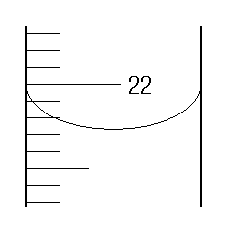
\includegraphics[width=0.25\textwidth]{Gradation.png}
		\caption{액체가 담긴 눈금 실린더의 눈금}
		\label{fig:gradation}
	\end{figure}
		
	\paragraph{유효숫자를 세는 규칙}
	\begin{itemize}
		\item 0이 아닌 숫자는 모두 유효숫자이다.
		\item 0이 아닌 숫자의 중간에 있는 0은 유효숫자이다.
		\item 첫 번째 0이 아닌 숫자 앞의 0은 유효숫자가 아니다.\\
		0은 유효숫자가 없다. 0.000이라도 유효숫자는 \unit{0}{개}이다.
		\item 소숫점 아래 마지막 0이 아닌 숫자 뒤의 0은 유효숫자이다.
		\item 자연수에서 마지막 0이 아닌 숫자 뒤의 0은 유효숫자인지
		알 수 없다. 반올림한 경우 앞에서부터 반올림받은 자리까지가
		유효숫자이다.
		\item 정의에 의해 성립된 값이나 세어서 구한 값처럼
		측정 기구를 사용하지 않는 모든 값은 완전수로서
		무한대의 유효숫자를 갖는 것으로 취급한다.
	\end{itemize}
	
	\paragraph{유효숫자의 연산}
	\begin{itemize}
		\item 덧셈과 뺄셈 : 계산 결과의 유효숫자는
		계산에 사용한 값 중 정밀도가 가장 낮은 측정값의
		유효숫자와 같다.
		$4.56 \times 1.4 = 6.38 \rightarrow 6.4$
		\item 곱셈과 나눗셈 : 계산 결과의 유효숫자는
		계산에 사용한 값 중 정밀도가 가장 낮은 측정값의
		유효숫자와 같다.
		$12.22+18.0+1.013=31.123 \rightarrow 31.1$
		\item 지수와 로그 : 자릿수를 의미하는 숫자는
		유효숫자에서 제외한다. 즉, 대수에서 소수점 이하의 개수는
		주어진 값의 유효숫자의 개수와 같다.
		$10^{2.345} = 2.21 \times 10^{2}$,
		$\log 12345 = 4.09149$
	\end{itemize}
	
	\paragraph{유효숫자를 고려한 반올림 규칙}
	\begin{itemize}
		\item 여러 단계의 계산을 연속해서 할 때는
		마지막 결과를 얻을 때까지 모든 숫자를 가져가 연산한 뒤
		마지막 결과 값에서 유효숫자의 개수를 고려하여 반올림한다.
		\item 반올림을 할 때는 마지막 유효숫자의
		첫 번째 오른쪽 숫자만을 사용한다.
		\item 최종 유효숫자가 맞춰지도록 행한다.
		만일 반올림하는 숫자가 5보다 작으면 버리고
		5 이상은 그 앞 자리 수에 1을 더한다.
	\end{itemize}
	
	\subsubsection{\boldmath 표준편차(standard deviation)}
	자료의 분산 정도를 나타내는 수치로 보통 기호는 $\sigma$를 쓴다.
	표준 편차가 작은 것은 평균값 주위로 분산 정도가 작다는 것을 의미한다.
	\begin{gather}
	\sigma = \sqrt{
		\frac{1}{n-1}\sum_{i=1}^{N}(x_{i}-\overline{x})^{2}
	} \label{eq:stdev}
	\end{gather}
	($n$ : 표본의 개수, $x_{i}$ : $i$번째 표본값,
	$\overline{x}$ : 표본평균)
	
	식 \ref{eq:stdev}에서 $n-1$로 나누는 것은 자유도의 개념이다.
	자유도 $v$에 대해 모수가 $k$개라면 자유도는 $v = n - k$로 정해진다.
	\cite{deg_free}
	
	상대 표준편차는 표준편차를 평균으로 나누어 구할 수 있다.
	
	\subsubsection{불확도(uncertainty)}
	불확도는 측정값의 의심할 수 있는 정도로
	모든 측정은 의심의 범위를 가진다.
	측정 불확도는 구간과 신뢰 수준으로 나타낸다.
	총 불확도는 불확도에 기여하는 각 요소에 의한 표준 불확도를 구한 뒤
	표준 불확도들의 제곱을 더한 값에 제곱근을 취하여 구한다.
	\cite{Stephanie_Bell}
	아날로그 눈금의 경우 최소 눈금 크기의 절반을 불확도로 하고,
	디지털 눈금의 경우 최소 눈금 크기를 불확도로 한다.
	
	\subsubsection{표준 불확도(standard uncertainty)}
	모든 기여 불확도는 표준 불확도로의 변환을 통해 같은 수준의 신뢰 수준으로
	표현되어야 한다. 표준 불확도는 그 크기가 $\pm\sigma$($\sigma$ : 
	불확도)로
	생각될 수 있는 범위이다. 표준 불확도는 평균의 불확도를 말해 준다.
	표준 불확도는 대개 $u$ 또는 $u(y)$($y$에 의한 표준 불확도)로 나타낸다.
	
	표준 불확도를 구하는 방법으로 Type A와 Type B가 있다.
	Type A는 통계학을 이용하여 구하는 것이고,
	Type B는 과거 측정값이나 알려진 정보 등 다른 정보를 이용하여 구하는 
	것이다.
	\cite{Stephanie_Bell}
			
	\paragraph{Type A 방법을 사용한 표준 불확도 계산}
	표본값이 가우시안 분포를 따른다는 가정 하에 계산하며,
	가정에 따르면 $t$-분포를 따른다고 할 수 있다.
	반복 측정값이 있을 때 Type A 방법을 사용한 표준 불확도는
	평균과 표준편차에 의해 결정된다. 평균의 불확도는
	식 \ref{eq:un}\로 계산된다.
	\begin{gather}
	u = \frac{\sigma}{\sqrt{n}} \label{eq:un}
	\end{gather}
	
	($\sigma$ : 표준편차, $n$ : 표본의 개수)
	
	평균의 불확도는 평균의 표준편차 또는 평균의 오차 등으로도 불렸다.
	\cite{Stephanie_Bell}
	
	\paragraph{Type B 방법을 사용한 표준 불확도 계산}
	정보가 더 부족한 경우, 불확정도의 상·하한값만을 알 수 있는 경우가 있다.
	자료가 균등 분포를 따른다고 가정할 수 있는 경우, 불확도는
	식 \ref{eq:un2}에 의해 얻어진다.
	\begin{gather}
	\frac{a}{\sqrt{3}} \label{eq:un2}
	\end{gather}
	
	($a$ : 상·하한 차의 절반)
	
	예를 들어 길이 눈금을 읽을 때, 실제 끝 눈금이 어디에 있을지는
	내가 읽은 눈금 주변 범위 내 모두 균일하다. 이러한 경우 Type B 방법을
	사용하여 표준 불확도를 계산한다.
	\cite{Stephanie_Bell}
	
	\subsubsection{범위 인자(coverage factor)}
	불확도가 $t$-분포를 따른다는 가정에 의하면 대푯값 전후로
	불확도 하나를 더하고 뺀 범위는 신뢰 수준이 \SI{68}{\percent}이다.
	따라서 신뢰 수준을 높이기 위해 불확도에 인자 $k$를 곱해
	확장된 불확도(주로 $U$로 표기)를 만든다. $k$가 2일 때
	신뢰 수준은 약 \SI{95}{\percent}가 된다.
	
	\subsubsection{상대 불확도(relative uncertainty)}
	불확도가 \SI{1}{\centi\metre}라고 할 때, 이 불확도로
	\SI{1}{\metre}의 측정에서는 정밀한 측정을 했다고 볼 수 있지만,
	\SI{3}{\centi\metre}의 측정에서는 정밀한 측정이라고 볼 수 없다.
	따라서 측정의 질은 불확도 자체에 연관된 것이 아닌 불확도와 대푯값의
	비에 연관되어 있다고 볼 수 있다. 상대 불확도 $u_{\mathrm{rel}}$은
	식 \ref{eq:un_rel}과 같다.
	\begin{gather}
	u_{\mathrm{rel}} = \frac{u}{|\text{대푯값}|} \label{eq:un_rel}
	\end{gather}
	
	상대 불확도는 정밀도(precision)라고 불리기도 한다.\cite{Taylor_John1}
	
	\subsubsection{불확도의 표현}
	불확도는 매우 정밀한 실험에서는 두 자리까지 나타내기도 하나
	보통은 한 자리까지 나타낸다. 다만 맨 앞 자릿수가 1인 경우,
	반올림하면 오차가 커지기 때문에 두 자리까지 나타내는 게 좋을 수 있다.
	불확도와 함께 대푯값을 나타낼 때는
	$\text{(대푯값)}\pm\text{(불확도)}$로 나타낸다.
	이때 단위를 각각 붙이지 않고 묶어서 한 번에 표시한다.
	
	대푯값의 마지막 자리는 불확도의 자리에 맞추어 표현해야 한다.
	예를 들어 대푯값이 81.3이고 불확정도가 3일 경우 표기는 $81.3\pm 3$이 
	아닌 $81\pm3$으로 표기하여야 하고, 불확정도가 0.03일 경우 $81.30\pm 
	0.03$으로 표기하여야 한다.
	\cite{Taylor_John2}
	
	\subsubsection{불확도의 연산}
	각 불확도가 독립적이고 불규칙적일 때 불확도는
	더하고 빼는 연산의 경우 각 절대 불확도의 제곱을 더한 뒤
	양의 제곱근을 취한 값이 최종 연산 값의 절대 불확도가 되고,
	곱하고 나누는 연산의 경우 각 상대 불확도의 제곱을 더한 뒤
	양의 제곱근을 취한 값이 최종 연산 값의 상대 불확도가 된다.
	불확도가 없는 상수를 곱했을 경우 불확도는 그 상수의 절댓값 배가 된다.
	\cite{Penn}
	
	\subsubsection{밀도}
	서로 물체들의 질량과 부피 사이의 차이점을 비교하는 데
	밀도(density, $D$)라는 단위를 사용한다.
	즉 어떤 물체의 질량을 $M$, 부피를 $V$라고 하면 밀도 $D=M/V$가 된다.
	거의 모든 물체는 가열하면 일반적으로 팽창하므로
	밀도는 온도에 따라서 변하게 된다.
	따라서 어떤 특정 온도에서 측정된 밀도는
	그보다 높은 온도에서는 감소하게 되는데
	그 이유는 질량에는 변화가 없지만 부피가 증가하기 때문이다.
	그러므로 밀도에 대한 정확한 표시를 하기 위해서는
	밀도 측정 시의 온도를 표시해 주어야 한다.
		
	\subsubsection{무게와 질량}
	\begin{itemize}
		\item 무게 : 중력의 크기로 용수철 저울이나 앉은뱅이 저울로 측정
		(단위 : \si{\newton}, \si{\kilo\gramforce})
		\item 질량 : 물체의 고유한 양으로, 양팔 저울이나
		윗 접시 저울로 측정 (단위 : \si{\gram}, \si{\kilo\gram})\\
		질량의 기준은 킬로그램 원기이다.
		\item 질량과 무게의 차이점 : 질량은 변하지 않지만
		무게는 장소에 따라 달라진다.
		같은 장소에서 무게는 질량에 비례한다. 
	\end{itemize}
	
	\subsection{유의 사항}
	\begin{itemize}
		\item 피펫에 용액을 채울 때는 공기가 빨려 들어가지 않도록
		피펫 끝이 항상 액체 속에 잠겨 있도록 해야 하며,
		필터 속으로 액체가 들어가는 일이 없도록 유의한다.
		\item 피펫에 남은 액체가 없도록 마지막 남은 방울을 빼내어 
		오차를 줄인다.
		\item 뷰렛의 끝에 공기 방울이 남아있으면
		콕을 빨리 열어 공기를 빼낸 후 사용한다.
		\item 뷰렛을 읽을 때는 첫 눈금과 나중 눈금의 차이를 통해
		읽도록 한다.
		\item 모든 눈금을 읽을 때는 눈높이로 맞추어 읽도록 한다.
	\end{itemize}
	
	\section{기구 및 시약}
	
	\subsection{실험 기구}
	\SI{50}{\milli\litre} 비커, \SI{10}{\milli\litre} 눈금 피펫,
	\SI{10}{\milli\litre} 홀 피펫, \SI{1000}{\micro\litre} 마이크로피펫,
	고무 필러, 다이얼식 필러, 전자 저울, 뷰렛, 깔때기, 스탠드,
	\SI{10}{\milli\litre} 눈금 실린더, 증류수, 온도계, 일회용 스포이트,
	피펫 팁, 동전, 바이알
	
	\subsection{실험 시약}
	물
	
	\section{실험 과정}
	
	\subsection{무게 측정}
	\begin{enumerate}
		\item 실험에 사용할 저울의 제조회사와 모델, 측정 용량(최대 측정 무게),
		측정의 정밀도를 조사하고 실험 결과에 적는다.
		\item 저울의 균형이 맞는지 확인해야 하며,
		저울의 올바른 사용법을 충분히 익힌 후 정지점을 결정한다.
		\item \SI{50}{\milli\litre} 비커를 깨끗이 씻어 말린 뒤
		무게를 달아 기록한다. 온도계로 온도를 측정한다.
	\end{enumerate}
	
	\subsection{피펫을 이용한 액체의 이동} \label{subsec:second}
	\begin{enumerate}
		\item \SI{10}{\milli\litre} 눈금 피펫과 \SI{10}{\milli\litre} 
		홀 피펫에 기재되어 있는 사항을 모두 기록한다.
		\item 두 종류의 피펫 필러(고무 필러 및 다이얼식 필러)의 사용법을
		숙지한 뒤 증류수를 피펫에 반 정도 채운 다음,
		피펫을 옆으로 기울여서 돌려가면서 피펫의 안쪽 면을 헹구어 준 뒤
		증류수를 버린다.
		\item 피펫의 최대 용량만큼 증류수를 취하여
		이미 무게를 측정한 비커에 옮겨 무게를 기록한다.\\
		(각각의 피펫에 대하여 5회씩 반복)
		\item 온도별 물의 밀도를 이용하여
		피펫으로 옮긴 증류수 부피의 평균값과 표준편차를 구한다.
		\label{itm:fourth}
		\item 눈금 피펫과 \SI{1000}{\micro\litre} 마이크로피펫으로
		정확하게 \SI{2.00}{\milli\litre}의 증류수를 취하여
		무게 측정하기를 $5\,\mbox{회}$ 반복한 뒤
		\ref{itm:fourth} 과정을 다시 실시한다.
	\end{enumerate}
	
	\subsection{눈금 실린더를 이용한 액체의 이동}
	\begin{enumerate}
		\item \SI{10}{\milli\litre} 눈금 실린더에 기재된 모든 사항을
		자세히 기록한 뒤 눈금 실린더를 안쪽 벽면에 물방울이 생기지 
		않도록 깨끗이 씻고 증류수로 헹군다.
		\item \SI{2.00}{\milli\litre}의 증류수를 채운 다음
		이미 무게를 측정한 비커에 옮겨 무게를 기록한다.(5회 반복)
		\item \ref{subsec:second}\과 같은 방법으로 옮긴 증류수 부피의 
		평균과 표준편차를 구한다.
	\end{enumerate}
	
	\subsection{뷰렛을 이용한 액체의 이동}
	\begin{enumerate}
		\item 뷰렛의 사용법과 눈금 읽는 법을 숙지한 뒤
		뷰렛에 기재된 모든 사항을 자세히 기록하고,
		깨끗하게 씻어서 헹군 뷰렛에 증류수를 채운다.
		\item \SI{2.00}{\milli\litre}의 증류수를 빼내어
		이미 무게를 측정한 비커에 옮겨 무게를 기록한다.(5회 반복)
		\item \ref{subsec:second}\과 같은 방법으로 옮긴 증류수 부피의 
		평균과 표준편차를 구한다.
	\end{enumerate}
	
	\subsection{동전의 밀도 구하기}
	\begin{enumerate}
		\item 눈금 실린더에 물을 넣고, 동전 \unit{15}{개}를 넣어
		증가한 물의 부피를 측정한다.
		\item 동전 \unit{15}{개}의 무게를 재서 15로 나누어
		동전 \unit{1}{개}의 무게를 측정한다.
		\item 두 값을 통해 밀도를 계산한다.
	\end{enumerate}
	
	\subsection{공기의 밀도 구하기}
	\begin{enumerate}
		\item 물을 꽉 채운 바이알의 무게를 측정한다.
		\item 물을 꽉 채운 상태에서 마이크로피펫을 이용해
		\SI{1}{\milli\litre}만큼의 물을 밖으로 세 번 따라낸 뒤
		뚜껑을 완전히 닫고 무게를 측정한다.
		\item 두 무게 차이를 구한 뒤 \SI{3}{\milli\litre}만큼의 물의 
		무게에서 뺀 값을 \SI{3}{\milli\litre}만큼을 공기의 무게로 
		계산하여 공기의 밀도를 구한다.
	\end{enumerate}
	
	\section{실험 결과}
	
	\subsection{무게 측정}
	실험에 사용한 전자 저울의 정보는 다음과 같다.
	\begin{itemize}
		\item 제조 회사 : OHAUS(미국)
		\item 눈금 : \SI{0.001}{\gram}
		\item 사용 범위 : \SIrange{0.04}{210}{\gram}
	\end{itemize}
	
	측정한 \SI{50}{\milli\litre} 비커의 무게, 물의 온도와
	물의 온도를 이용하여 구한 물의 밀도는 다음과 같다.
	\begin{itemize}
		\item 비커 무게 : \SI{38.749}{\gram}
		\item 물의 온도 : \SI{15.9}{\degreeCelsius}
		\item 물의 밀도 : \SI{0.998959}{\gram\per\milli\litre} 
		\cite{Santa_Cruz}
	\end{itemize}

	
	\subsection{피펫을 이용한 액체의 이동} \label{sbsec:pip}
	실험에 사용한 \SI{10}{\milli\litre} 눈금 피펫의 정보는 다음과 같다.
	\begin{itemize}
		\item 제조 회사 : OMG
		\item 최대 용량 : \SI{10}{\milli\litre}
		\item 오차 범위 :
		In \SI{20}{\degreeCelsius}, \SI{+-0.04}{\milli\litre}
		\item B/Ex(TD)
	\end{itemize}
	
	실험에 사용한 \SI{10}{\milli\litre} 홀 피펫의 정보는 다음과 같다.
	\begin{itemize}
		\item 제조 회사 : PROLINE
		\item 사용 범위 : \SIrange{100}{1000}{\micro\litre}
		\item 조작 단위 : \SI{5}{\micro\litre}
		\item (Biohit)
	\end{itemize}
	
	피펫을 이용해 비커에 물을 옮긴 뒤 측정한 비커의 무게와 그 평균,
	평균의 표준편차는 표 \ref{tab:data1}\과 같다.
	\begin{table}[H]
		\centering
		\begin{tabular}{l c c c c c c c}
			\thickhline
			사용 기구(측정량) & 1회 & 2회 & 3회 & 4회 & 5회 &
			평균 & \makecell{평균의\\표준편차} \\
			\hline
			눈금 피펫(\SI{10}{\milli\litre}) &
			48.728 & 48.662 & 48.723 & 48.685 &
			48.734 & 48.706 & 0.014 \\
			홀 피펫(\SI{10}{\milli\litre})&
			48.640 & 48.626 & 48.662 & 48.665 &
			48.646 & 48.648 & 0.007 \\
			눈금 피펫(\SI{2}{\milli\litre}) &
			40.724 & 40.723 & 40.711 & 40.703 &
			40.695 & 40.711 & 0.006 \\
			마이크로 피펫(\SI{2}{\milli\litre}) &
			40.750 & 40.743 & 40.745 & 40.764 &
			40.754 & 40.751 & 0.004 \\
			\thickhline
		\end{tabular}
		\caption{피펫을 이용해 물을 옮긴 뒤 측정한
			비커의 무게(단위 : \si{\gram})}
		\label{tab:data1}
	\end{table}

	최소 눈금 단위를 고려하면 질량을 잴 때
	눈금에 따른 불확도는 \SI{0.001}{\gram}이다.
	
	통계학적 불확도인 평균의 표준편차를 $u_{\mathrm{ran}}$,
	눈금에 따른 불확도를 $u_{\mathrm{sys}}$라고 할 때
	옮긴 물 무게의 총 불확도
	$u(m) = \sqrt{{u_{\mathrm{ran}}}^2 + 2{u_{\mathrm{sys}}}^2}$이다.
	(눈금의 불확도는 처음 잴 때와 옮긴 뒤 잴 때 각각 발생하므로
	두 배 해주어야 한다)
	
	나중 비커 무게의 평균에서 처음 비커 무게를 뺀 값을 $m$이라고 할 때,
	상대 불확도는 $u(m) / m$이다.
	
	옮긴 물의 부피 $V = m / d$($d$ : 밀도)이다.
	물의 밀도의 불확도는 매우 작아 무시할 수 있는 수준이므로
	고려하지 않는다.
	옮긴 물 부피의 상대 불확도는 옮긴 물 무게의 상대 불확도와 같다.
	피펫의 종류에 따른 옮긴 물 부피의 오차의 절댓값과 상대 오차,
	표준 절대 불확도, 상대 불확도는 표 \ref{tab:calc1}\과 같다.
	\begin{table}[H]
		\centering
		\begin{tabular}{l D..{1.3} D..{1.2} D..{1.3} D..{1.2}}
			\thickhline
			사용 기구(측정량) &
			\multicolumn{1}{c}{오차(\si{\milli\litre})} &
			\multicolumn{1}{c}{상대 오차(\%)} &
			\multicolumn{1}{c}{불확도(\si{\milli\litre})} &
			\multicolumn{1}{c}{상대 불확도(\%)} \\
			\hline
			눈금 피펫(\SI{10}{\milli\litre}) &
			0.053 & 0.53 & 0.014 & 0.14 \\
			홀 피펫(\SI{10}{\milli\litre}) &
			0.112 & 1.12 & 0.007 & 0.07 \\
			눈금 피펫(\SI{2}{\milli\litre}) &
			0.040 & 2.0 & 0.006 & 0.3 \\
			마이크로 피펫(\SI{2}{\milli\litre}) &
			0 & 0 & 0.004 & 0.2 \\
			\thickhline
		\end{tabular}
		\caption{물의 밀도와 무게로 계산한
			피펫을 이용하여 옮긴 물의 부피}
		\label{tab:calc1}
	\end{table}
	
	\subsection{눈금 실린더를 이용한 액체의 이동}
	비커에 \SI{10}{\milli\litre} 눈금 실린더를 이용해
	\SI{2}{\milli\litre}의 물을 옮긴 뒤 측정한 값은
	표 \ref{tab:data2}\과 같다.
	\begin{table}[H]
		\centering
		\begin{tabular}{l c c c c c c c}
			\thickhline
			사용 기구(측정량) & 1회 & 2회 & 3회 & 4회 & 5회 &
			평균 & \makecell{평균의\\표준편차} \\
			\hline
			눈금 실린더(\SI{2}{\milli\litre}) &
			40.602 & 40.612 & 40.631 & 40.654 &
			40.674 & 40.635 & 0.013 \\
			\thickhline
		\end{tabular}
		\caption{눈금 실린더를 이용해 물을 옮긴 뒤 측정한
			비커의 무게(단위 : \si{\gram})}
		\label{tab:data2}
	\end{table}

	\ref{sbsec:pip}와 같은 과정을 거쳐 계산한 눈금 실린더를 이용하여 옮긴
	물 부피의 오차의 절댓값과 상대 오차, 표준 절대 불확도, 상대 불확도는
	표 \ref{tab:calc2}\과 같다.
	
	\begin{table}[H]
		\centering
		\begin{tabular}{l c c c c}
			\thickhline
			사용 기구(측정량) &
			오차(\si{\milli\litre}) &
			상대 오차(\%) &
			불확도(\si{\milli\litre}) &
			상대 불확도(\%) \\
			\hline
			눈금 실린더(\SI{2}{\milli\litre}) &
			0.114 & 5.82 & 0.013 & 0.7 \\
			\thickhline
		\end{tabular}
		\caption{물의 밀도와 무게로 계산한
			눈금 실린더를 이용하여 옮긴 물의 부피}
		\label{tab:calc2}
	\end{table}
	
	\subsection{뷰렛을 이용한 액체의 이동}
	실험에 사용한 뷰렛의 정보는 다음과 같다.
	\begin{itemize}
		\item 제조 회사 : 새한
		\item 최대 용량 : \SI{50}{\milli\litre}
		\item TD \SI{20}{\degreeCelsius}
	\end{itemize}
	
	비커에 뷰렛을 이용해 \SI{2}{\milli\litre}의 물을 옮긴 뒤 측정한 값은
	표 \ref{tab:data3}\과 같다.
	\begin{table}[H]
		\centering
		\begin{tabular}{l c c c c c c c}
			\thickhline
			사용 기구(측정량) & 1회 & 2회 & 3회 & 4회 & 5회 &
			평균 & \makecell{평균의\\표준편차} \\
			\hline
			뷰렛(\SI{2}{\milli\litre}) &
			40.792 & 40.784 & 40.725 & 40.654 &
			40.750 & 40.74 & 0.02 \\
			\thickhline
		\end{tabular}
		\caption{뷰렛을 이용해 물을 옮긴 뒤 측정한
			비커의 무게(단위 : \si{\gram})}
		\label{tab:data3}
	\end{table}
	
	\ref{sbsec:pip}와 같은 과정을 거쳐 계산한 뷰렛을 이용하여 옮긴
	물 부피의 오차의 절댓값과 상대 오차, 표준 절대 불확도, 상대 불확도는
	표 \ref{tab:calc3}\과 같다.
	
	\begin{table}[H]
		\centering
		\begin{tabular}{l c c c c}
			\thickhline
			사용 기구(측정량) &
			오차(\si{\milli\litre}) &
			상대 오차(\%) &
			불확도(\si{\milli\litre}) &
			상대 불확도(\%) \\
			\hline
			뷰렛(\SI{2}{\milli\litre}) &
			0.01 & 0.5 & 0.02 & 1.2 \\
			\thickhline
		\end{tabular}
		\caption{물의 밀도와 무게로 계산한 뷰렛을 이용하여 옮긴 물의 부피}
		\label{tab:calc3}
	\end{table}
	
	\subsection{동전의 밀도 구하기}
	측정한 동전 $15\,\mbox{개}$의 질량과 부피, 그리고 이를 이용해 구한
	동전의 밀도는 다음과 같다.
	\begin{itemize}
		\item 부피 : \SI{9.0}{\milli\litre}
		\item 질량 : \SI{81.021}{\gram}
		\item 밀도 : \SI{9.0}{\gram\per\milli\litre}
	\end{itemize}
	
	\subsection{공기의 밀도 구하기}
	측정한 물을 꽉 채운 초기 상태의 바이알과 물 \SI{3}{\milli\litre}를 뺀
	바이알의 무게, 그리고 그를 이용하여 계산한 공기의 밀도는 다음과 같다.
	\begin{itemize}
		\item 물을 꽉 채운 바이알의 무게 : \SI{21.661}{\gram}
		\item 물 \SI{3}{\milli\litre}를 뺀 바이알의 무게 :
		\SI{18.626}{\gram}
		\item 공기의 밀도 : \SI{0.011}{\femto\gram\per\milli\litre}
	\end{itemize}
	
	\section{관찰 및 토의}
	
	\subsection{실험 기구 기재 사항 정보}
	전자 저울에 기재된 사항의 의미는 다음과 같다.
	\begin{itemize}
		\item 눈금 : 측정할 수 있는 무게의 정밀도이다.
		이 실험에 사용한 저울은 \SI{0.001}{\gram}까지 측정이 가능하다.
		\item 사용 범위 : 잴 수 있는 무게의 최소치와 최대치를
		표시한 것이다.
		이 실험에 사용한 저울은 \SIrange{0.04}{210}{\gram} 범위에서
		무게 측정이 가능하였다.
	\end{itemize}
	
	피펫에 기재된 사항의 의미는 다음과 같다.
	\begin{itemize}
		\item B : Class B를 의미하는 것으로,
		부피 허용 오차가 DIN과 ISO의 기준에 맞는 제품인
		A/AS Class 허용 오차의 두 배라는 뜻이다.
		\item TD : 표시된 눈금까지 피펫 내부에 들어있는 부피를
		자연 방출 시간에 따라 밖으로 자연 방출시켰을 때
		빠져나온 용액의 부피를 말하기 때문에
		자연 방출 시간만 지켜서 용액을 방출시키면 그 부피만큼 옮겨진다.
		자연 방출 시간 후 피펫 끝 속에 남아있는 마지막 한 방울을
		입으로 불어내지 않아도 된다. TC는 그 반대의 의미로
		불어내야 한다.
		\item In \SI{20}{\degreeCelsius}, \SI{+-0.080}{\milli\litre} :
		\SI{20}{\degreeCelsius}에서 가장 정밀하며,
		그 때의 오차가 \SI{+-0.080}{\milli\litre}이라는 의미이다.
	\end{itemize}
	
	\subsection{피펫의 종류에 따른 액체 이동 비교}
	같은 \SI{10}{\milli\litre}를 옮긴 눈금 피펫과 홀 피펫의
	평균 표준편차 값을 비교하면 홀 피펫이 더 작다.
	이를 통해 홀 피펫이 눈금 피펫보다 더 정밀도가 높음을 알 수 있다.
	이는 홀 피펫은 가운데 부분을 두껍게 하여 눈금을 읽는 부분의 지름이
	눈금 피펫보다 더 작은데, 이로 인해 부피 차이에 따른 높이 변화가 더 커
	차이를 더 잘 관찰할 수 있기 때문이다.
	
	같은 \SI{2}{\milli\litre}를 옮긴 눈금 피펫과 마이크로 피펫의
	오차를 비교하면 마이크로 피펫이 더 작다.
	또한, 표준편차 역시 마이크로 피펫이 더 작다.
	이를 통해 마이크로 피펫이 눈금 피펫보다
	정확도와 정밀도가 더 높음을 알 수 있다.
	정확도와 정밀도가 높은 이유는 사람이 눈금을 읽어 부피를 측정해야 하는
	눈금 피펫과 달리 마이크로 피펫은 기계가 설정한 부피를 빨아올리기 때문에
	더 정확하고 정밀한 측정을 할 수 있어서이다.
	
	같은 눈금 피펫을 이용하여 \SI{10}{\milli\litre}와 \SI{2}{\milli\litre}를
	옮기는 실험에서 절대 오차와 불확도는 비슷하나 적은 양을 옮긴 경우의
	상대 오차와 불확도가 더 크다. 이는 같은 크기의 오차를 발생시키는 경우
	적은 양일 때 상대적인 변동의 크기가 더 크기 때문이다.
	
	\subsection{실험 기구에 따른 액체 이동 비교}
	같은 \SI{2}{\milli\litre}를 옮긴 눈금 피펫, 마이크로 피펫,
	눈금 실린더, 뷰렛의 경우 불확도는 뷰렛, 눈금 실린더, 눈금 피펫,
	마이크로 피펫 순으로 높았다. 이는 실험 기구의 안쪽 반지름
	크기 순서와 일치한다. 안쪽 반지름이 클수록 부피에 따른 높이 변화가
	적어 더 관찰하기 어렵기 때문에 불확도가 커지게 된다.
	추가로 뷰렛은 다른 기구와 달리 눈금을 두 번(시작 눈금과 끝 눈금)
	읽기 때문에 불확도가 더 커진다.
	
	제일 오차가 컸던 기구는 눈금 실린더였다. 이는 눈금 실린더는
	출용(to deliver, TD)이 아닌 수용(to contain, TC)이기 때문에
	눈금 실린더로 액체를 옮기면 액체 일부가 실린더에 남아 전부 옮겨지지
	않기 때문이다.
	
	\subsection{동전의 밀도}
	실험에 사용한 동전의 주 원료는 구리와 니켈이다.
	동전의 정확한 밀도를 알 수 없어 구리와 니켈의 밀도
	약 \SI{8.9}{\gram\per\cubic\centi\metre}를 실제 동전의 밀도로 가정한다.
	
	실험에서 구한 밀도는 실제 동전의 밀도와 상당히 비슷하였다.
	
	\subsection{공기의 밀도}
	ISA에 따르면 수면에서 \SI{15}{\degreeCelsius} 공기의 밀도는
	약 \SI{1.225}{\milli\gram\per\cubic\centi\metre}이다.
	실험을 통해 구한 값은 이보다 상당히 작다.
	이는 실험 설계가 잘못되었음을 보여 주며,
	실험을 통해 나온 양수 값은 실험 오차로 인해 나온 값일 것이다.
	
	\section{결론 및 제언}
	\begin{itemize}
		\item 실험 기구와 측정하는 양에 따라 오차와 불확도가 달라진다.
		실험을 할 때에는 상황에 맞는 올바른 기구를 사용하도록 하고,
		가급적 한 번에 많이 측정하여 측정 횟수를 줄이는 것이
		오차와 불확도를 줄일 수 있을 것이다.
		\item 실험에서 전자 저울의 최소 눈금에 따른 불확도는 최종 
		불확도에 영향을 미치지 않을 만큼 작았다. 추후 불확정도를 계산할 
		때에도 편차가 크지 않다면 고려하지 않아도 될 것 같다.
		\item 대기압 하에서 공기는 공기만큼의 부력을 받기 때문에
		대기압과 같은 압력의 공기를 저울로 측정하면 무게는 0이 된다.
		따라서 속이 빈 고무공과 같은 물건에 주사기를 이용하여 대기압과 
		같은 공 내부에 일정 부피의 공기를 집어넣어 측정하는 방법이
		적절하다고 생각된다. \cite{kimandjang}
	\end{itemize}
	
	\begin{thebibliography}{00}
		\bibitem{deg_free} David C. Stone \& Jon Ellis (2008),
		``Stats Tutorial - Instrumental Analysis and Calibration'',
		경기과학고등학교에서 2016년 1월 18일 검색,
		웹 주소 :
		http://www.chem.utoronto.ca/\allowbreak
		coursenotes/analsci/stats/DegFree.html
		\bibitem{Stephanie_Bell} Stephanie Bell (1999),
		``Measurement Good Practice Guide No. 11 (Issue 2)'',
		경기과학고등학교에서 2016년 1월 18일 검색,
		웹 주소 : http://publications.npl.co.uk/npl\_web/pdf/mgpg11.pdf
		\bibitem{Taylor_John1} John R. Taylor,
		An introduction to error analysis (2nd ed.), 1997, pp.28-29
		\bibitem{Taylor_John2} John R. Taylor,
		An introduction to error analysis (2nd ed.), 1997, pp.14-16
		\bibitem{Penn} Department of Physics \& Astronomy of
		University of Pennsylvania, ``Averaging, Errors and
		Uncertainty'', 경기과학고등학교에서 2016년 1월 18일 검색,
		웹 주소 : http://\allowbreak virgo-physics.sas.upenn.edu/\allowbreak
		uglabs/\allowbreak lab\_manual/\allowbreak Error\_Analysis.pdf
		\bibitem{Santa_Cruz} Department of Chemistry at the University 
		of California, Santa Cruz, ``Lab 1 - Density Determinations and 
		Various Methods to Measure Volume'', 경기과학고등학교에서 
		2016년 1월 18일 검색, 웹 주소 :
		http://\allowbreak www.webassign.net/\allowbreak
		labsgraceperiod/\allowbreak ucscgencheml1/\allowbreak
		lab\_1/\allowbreak images/\allowbreak figure6.png
		\bibitem{kimandjang} 김재경, 장용성,
		"공기질량 측정실험의 개선에 관한 연구",
		과학수학교육연구, 제14권, pp.5-11, 1990
	\end{thebibliography}
			
\end{document}